\documentclass{swfcthesis}

\renewcommand{\acknowledgmentspage}{% Acknowledgments page  
  \phantomsection%
  \addcontentsline{toc}{chapter}{Acknowledgments}
  \chapter*{Acknowledgments}

  I would like to thank my supervisor Mr. WANG Xiaolin for his continuous support of my
  four years undergraduate study. I am extremly thankful to him for sharing expertise, and
  sincere and valuable guidance and encouragement extended to me.
  
  \fxerror{You translate the following in English.}
  
  我最想感谢的是我的女友,她容忍我在完成这个设计时
  的很多个夜晚不陪她,给我支持,鼓励我,不抱怨。所以我愿意把这个简单操作系统命名为RongOS,
  蓉便是她名字的最后一个字。谢谢你,我最亲爱的。}

\renewcommand{\advisorinfopage}{% Advisor info page
  \phantomsection%
  \addcontentsline{toc}{chapter}{Supervisor}
  \chapter*{Supervisor}
  Xiaolin WANG (Mr.), 49 years old, got his MSc degree at University of Greenwich in
  UK\@. Currently he's been working as a lecturer at the School of Big Data and
  Intelligence Engineering, Southwest Forestry University in China, teaching Linux,
  Operating Systems, and Computer Networking.
  \clearpage}

\renewcommand{\contentsname}{Contents}
\renewcommand{\listfigurename}{List of Figures}
\renewcommand{\listtablename}{List of Tables}
\renewcommand{\figurename}{Fig.}
\renewcommand{\tablename}{Table}
\renewcommand{\listingscaption}{Code} % used by minted
\renewcommand{\listoflistingscaption}{List of Codes}

\addbibresource{thesis.bib}

\begin{document}

\Title{RongOS --- 一个简单操作系统的设计与实现}
\Author{蒲启元}
\Advisor{王晓林}
\AdvisorTitle{讲师}
\Month{六}
\Year{二〇一八}

\Subject{计算机科学与技术专业} %专业名称(比如 电子信息工程专业)

\Abstract{操作系统管理着计算机的硬件和软件资源,它是向上层应用软件提供服务(接口)的核心系
  统软件,这些服务包括进程管理,内存管理,文件系统,网络通信,安全机制等。操作系统的设计与
  实现则是软件工业的基础。为此,在国务院提出的《中国制造2025》中专门强调了操作系统的开
  发\cite{china_2025}。但长期以来,操作系统核心开发技术都掌握在外国人手中,技术受制,对于我
  们的软件工业来说很不利。本项目从零开始设计开发一个简单的操作系统,包括boot loader,中断,
  内存管理,图形接口,多任务等功能模块,以及能运行在这个系统之上的几个小应用程序。尽管这
  个系统很简单,但它是自主开发操作系统的一次尝试。}

\Keywords{操作系统,进程,内存,中断,boot loader}

\enTitle{RongOS --- A simple OS implementation}

\enAuthor{Qiyuan PU}

\enAbstract{Operating system manages the hardware and software resources in a running
  computer system. It is the core of any modern software system and provides services
  (interfaces) to upper layer applications. The services it provides include process
  management, memory management, file system, network communication, security mechanism
  and more. Operating system development is the foundation and core of software
  industry. Therefore, \emph{Made in China 2025} emphasizes the development of operating
  system that put forward by The State Council of China. For long time, however, the OS
  kernel development technology is dominated by foreigners. This technical limitation is
  detrimental to the development of our software industry. In this project, we presents a
  simple operating system which includes a boot loader, interrupt services, memory
  management functions, a graphic interface, and multi-process management functions. Also,
  some trivial user-level applications are provided for system testing purpose. This
  simple toy OS is an experimental trial for developing an operating system from scratch.}

\enKeywords{operating system, boot loader, interrupt, process management, memory management}

%%% 下面六行不要动!
\makepreliminarypages% 封面
\frontmatter          
\tableofcontents     % 目录
\listoffigures       % 插图目录
\listoftables        % 表格目录
\listoffixmes{}

\mainmatter{}

\chapter{Introduction}

\section{Background}

Contemporary software systems are beset by problems that create challenges and
opportunities for broad new OS research. There are five areas could improve user
experience including dependability, security, system configuration, system extension, and
multiprocessor programming.

The products of forty years of OS research are sitting in everyone's desktop computer,
cell phone, car, etc., and it is not a pretty picture.  Modern software systems are
broadly speaking complex, insecure, unpredictable, prone to failure, hard to use, and
difficult to maintain. Part of the difficult is that good software is hard to write, but
in the past decade, this problem and more specific shortcomings in systems have been
greatly exacerbated by increased networking and embedded systems, which placed new demands
that existing architectures struggled to meet. These problems will not have simple
solutions, but the changes must be pervasive, starting at the bottom of the software
stack, in the operating system.

The world needs broad operating system research. Dependability, security, system
configuration, system extension, and multi-processor programming illustrate areas were
contemporary operating systems have failed to meet the software challenges of the modern
computing environment\cite{hunt2005broad}.


\section{Preliminary Works}

\subsection{Development Environment}

\begin{description}
\item[OS platform:] Debian 9, Linux kernel 4.12.0-1-amd64
\item[Editor:] GNU Emacs 25.2.2
\item[Run time VM:] QEMU emulator 2.8.1
\item[Assembler:] Nask
\item[Compiler:] CC1(Based on gcc)
\item[Debugger:] GNU gdb 7.12
\item[Version Control:] git 2.15
\end{description}

\subsection{Tools}

Some tools were used to develop RongOS, \xout{see tools}\fxerror{need some descriptions
  about the
  tools}\footnote{\url{https://github.com/Puqiyuan/RongOS/tree/master/Tools}}. Note that
these tools are Windows executables \fxerror{(so what?)}. Among these tools, the most
important ones are:

\begin{description}
\item[nask.exe:] the assembler, a modified version of NASM\cite{30_os}
\item[cc1:] the C compiler
\end{description}

\subsection{Platform Setup}

The development platform (mainly the Debian system) was set up by following the
\emph{Debian Installation
  tutorial}\footnote{\url{http://cs2.swfc.edu.cn/~wx672/lecture_notes/linux/install.html}}. The
main steps include:
\begin{enumerate}
\item Installing the base Debian system;
\item Installing necessary software tools, such as emacs, web browser, qemu, wine, etc.;
\item Cloning configuration files by following the tutorial mentioned above;
\item Some more fine tweaks to satisfy my personal needs.
\end{enumerate}

\subsubsection{Qemu}

QEMU is a generic and open source machine emulator and virtualizer\cite{wiki:qemu}. In
this project, QEMU was used as the test bed.

Installing QEMU for my x86\_64 architecture can be easily done by executing the following
command:
\begin{verbatim}
     $ sudo apt-get install qemu-system-x86_64
\end{verbatim}

\subsubsection{Wine}

Wine (originally an acronym for ``Wine Is Not an Emulator'') is a compatibility layer
capable of running Windows applications on several POSIX-compliant operating systems, such
as Linux, macOS, and BSD\cite{wiki:wine}.

Because the tools I used in this project are in Windows executable format, so on Debian system,
Wine is needed to be installed:

\begin{verbatim}
     $ sudo apt-get update
     $ sudo apt-get install wine
\end{verbatim}

\subsubsection{Debian i386 support}

On 64-bit systems you need to enable multi-arch support for running 32-bit Windows
applications (many modern apps are still 32-bit, also for large parts of the Windows
subsystem itself). Our development tools were 32-bit Windows applications, so we needed to
have i386 support for our 64-bit Linux system.

\begin{verbatim}
     $ sudo dpkg --add-architecture i386
     $ sudo apt-get update
\end{verbatim}

\chapter{Leading Knowledge}
\label{cha:leading-knowledge-1}

\section{Layers}
\label{sec:layers}

\section{Memory Management}
\label{sec:memory-management}

\subsection{Overview}
\label{sec:overview}

\subsection{Round Down/Up and Page Size}
\label{sec:round-downup-page}


\section{Mouse}
\label{sec:mouse}

\section{The Leap --- Road to the 32 Bit Mode}
\label{sec:leap-road-32}

\section{Data Structure}
\label{sec:data-structure}

\section{Programmable Interrupt Controller}

\section{C Language Basic}

\section{Segments and Descriptors}

\section{Instruction Set}

An instruction set architecture (ISA) is an abstract model of a computer. It is also
referred to as architecture or computer architecture. An ISA defines everything a machine
language programmer needs to know in order to program a computer.

An ISA may be classified in a number of different ways. A common classification is by
architectural complexity. A complex instruction set computer (CISC) has many specialized
instructions, some of which may only be rarely used in practical programs. A reduced
instruction set computer (RISC) simplifies the processor by efficiently implementing only
the instructions that are frequently used in programs, while the less common operations
are implemented as subroutines, having their resulting additional processor execution time
offset by infrequent use.

On traditional architectures, an instruction includes an opcode that specifies the
operation to perform, such as add contents of memory to register—and zero or more operand
specifiers, which may specify registers, memory locations, or literal data\cite{wiki:isa}.

This simple RongOS is based on x86 architecture, the following instructions are commonly
used in programming RongOS:%

\begin{description}
\item[db:] the abbreviation of define byte, write a byte, also 8 bits to file.
\item[resb:] the abbreviation of reserve byte, reserved bytes and filling \texttt{0x00} in these reserved space.
\item[dw:] the abbreviation of define word, write two bytes, also 16 bits to file.
\item[dd:] the abbreviation of define double-word, write four bytes, also 32 bits to file.
\item[org:] load the program to specified address.
\item[jmp:] jump to another instruction.
\item[mov:] assign the right value to left variable.
\item[jc:] the abbreviation of jump if carry, it means if carry flag is 1, jump.
\item[jnc:] jump if not carry.
\item[jae:] jump if above or equal.
\item[jbe:] jump if below or equal.
\item[jb:] jump if below.
\item[equ:] equ is the abbreviation of equal.
\item[ret:] end of function, return.
\item[in:] get signal from device.
\item[out:] send signal to device.
\item[cli:] clear interrupt flag, set it to 0.
\item[sti:] set interrupt flag, set it to 1.
\item[pushfd:] push flags double-word.
\item[popfd:] pop flags double-word.
\item[lgdt:] load content from specified memory to initialize GDT (global descriptor table)
  register.
\item[lidt:] load content from specified memory to initialize IDT (interrupt descriptor
  table) register.
\end{description}

\section{x86 Registers}

In computer architecture, a processor register is a quick accessible location available
to a computer's central processing unit (CPU). Registers usually consist of a small amount
of fast storage, although some registers have specific hardware functions, and may be
read-only or write-only.  Almost all computers, whether load/store architecture or not,
load data from a larger memory into registers where it is used for arithmetic operations
and is manipulated or tested by machine instructions. Manipulated data is then often
stored back to main memory, either by the same instruction or by a subsequent one. Modern
processors use either static or dynamic RAM as main memory, with the latter usually
accessed via one or more cache levels\cite{wiki:registers}.

Processor registers are normally at the top of the memory hierarchy, and provide the
fastest way to access data. The term normally refers only to the group of registers that
are directly encoded as part of an instruction, as defined by the instruction
set. Registers are normally measured by the number of bits they can hold, for example, an
``8-bit register'' or a ``32-bit register''. For x86 architecture, the following registers
exist:

\begin{multicols}{3}
  \begin{description}
  \item[ax:] accumulator
  \item[bx:] base
  \item[cx:] counter
  \item[dx:] data
  \item[bl:] base low
  \item[al:] accumulator low
  \item[cl:] counter low
  \item[dl:] data low
  \item[bh:] base high
  \item[ah:] accumulator high
  \item[ch:] counter high
  \item[dh:] data high
  \item[sp:] stack pointer
  \item[bp:] base pointer
  \item[si:] source index
  \item[di:] destination index
  \item[es:] extra segment
  \item[cs:] code segment
  \item[ss:] stack segment
  \item[ds:] data segment
  \item[fs:] no name
  \item[gs:] no name
  \end{description}
\end{multicols}

Among these registers, \texttt{bx, bp, si} and \texttt{di} can be used to specify the
address of memory. But \texttt{ax, cx, dx} and \texttt{sp} can not.  \fxerror*{don't
  understand.}{When mov instruction is used, the number of bits of operation number should
  be the same}.
\begin{description}
\item[16-bit registers:] \texttt{ax, cx, dx, bx, sp, bp, si, di, es, cs, ss, ds}, and \texttt{fs}.
\item[8-bit registers] \texttt{al, cl, dl, bl, ah, ch, dh}, and \texttt{bh}.
\end{description}
Actually, as shown in Fig.~\ref{fig:regs}, all these 8-bit registers are parts of
corresponding 16-bit registers.

\begin{figure}[!htbp]
  \centering
  \begin{center}
    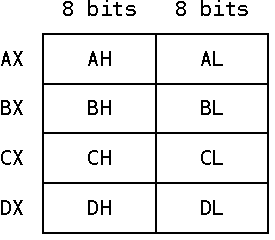
\includegraphics[width=.4\textwidth]{registers}
  \end{center}
  \caption{x86 registers}
  \label{fig:regs}
\end{figure}

\section{Interrupt Call}

BIOS interrupt calls perform hardware control or I/O functions requested by a program,
return system information to the program, or do both. A key element of the purpose of BIOS
calls is abstraction. The BIOS calls perform generally defined functions, and the specific
details of how those functions are executed on the particular hardware of the system are
encapsulated in the BIOS and hidden from the program\cite{wiki:bios-int}. The interrupt
calls are commonly used in RongOS are listed in Table~\ref{tbl:intcall}.

\begin{table}[!ht]
  \centering\tabulinesep=2mm
  \begin{tabu}{X[l,m,-1]X[l,m]X[-1,l,m]X[-1,l,m]}
    \tabucline-\rowfont\bfseries
    Interrupt\par{}Number & Register Parameter & Return Value & Function\\ \tabucline-
    0x10 &
    ah=0x0e(write character in tty mode)\par{}
    al=character code\par{}
    bh=0, bl=colorcolor& null & video services \\\tabucline-
    0x13 &
    ah=0x02(read sectors)\par{}
    ah=0x03(write sectors)\par{}
    ah=0x04(verify sectors)\par{}
    ah=0x0c(seek to specified track)\par{}
    al=number of sectors processing\par{}
    ch=cylinder \& 0xff  cl=sector number\par{}
    dh=header number dl=driver number\par{}
    es:bx=buffer address &
    FLACS.CF=0\par{}
    no error, ah = 0\par{}
    FLAGS.CF=1\par{}
    error, ah=error number\par{}& disk services \\ \tabucline-
  \end{tabu}
  \caption{RongOS interrupt calls}\label{tbl:intcall}
\end{table}

\section{Memory Map}

In the boot process, a memory map is passed on from the firmware in order to instruct an
operating system kernel about memory layout. It contains the information regarding the
size of total memory, any reserved regions and may also provide other details specific to
the architecture\fxerror{need citation}. For loading RongOS to memory, the memory layout
should be clarified as in Table~\ref{tbl:memlayout}.

\begin{table}[!ht]
  \centering\tabulinesep=2mm
  \begin{tabu}{%
      >{\texttt\bgroup}r<{\egroup}@{\,--\,}>{\texttt\bgroup}l<{\egroup}%
      >{\texttt\bgroup}r<{\egroup}@{\,--\,}>{\texttt\bgroup}l<{\egroup}%
      >{\texttt\bgroup}l<{\egroup}l}%
    \tabucline-\rowfont\bfseries%
    \multicolumn{2}{l}{Range (in hexadecimal)} &%
    \multicolumn{2}{l}{Range (in decimal)} &%
    \multicolumn{1}{l}{Size (in bytes)} & Usage \\ \tabucline-
    0000 & 03ff & 0000 & 1023 & 1024 &  interrupt vector table \\ 
    0400 & 04ff & 1024 & 1279 & 256 & BIOS data area \\ 
    0500 & 051f & 1280 & 1311 & 32 & Reserved \\ 
    0520 & 7bff & 1312 & 31743 & 30432 & conventional memory \\ 
    7c00 & 7dff & 31744 & 32255 & 512 & master boot record \\ 
    7e00 & 9ffff & 32256 & 655359 & 623104 & conventional memory \\ 
    a0000 & affff & 655360 & 720895 & 64K & VGA graphics RAM \\ 
    b0000 & b7fff & 720896 & 753663 & 32K & monochrome text mode \\ 
    b8000 & bffff & 753664 & 786431 & 32K & color text mode \\ 
    c0000 & c7fff & 786432 & 819199 & 32K & VGA video ROM \\ 
    c8000 & cbfff & 819200 & 835583 & 16K & IDE hard drive \\ 
    cc000 & cffff & 835584 & 851967 & 16K & optional adapter \\ \tabucline-
  \end{tabu}
  \caption{RongOS Memory Layout}\label{tbl:memlayout}
\end{table}

\section{Floppy Disk}

There are many ways to boot an operating system, from hard disk, USB, floppy disk, etc.
The structure of floppy disk is simple and for this simple operating system it's enough.

Fig.~\ref{fig:flpy1.png} shows the inside of a floppy disk:
\begin{figure}[!ht]
  \centering
  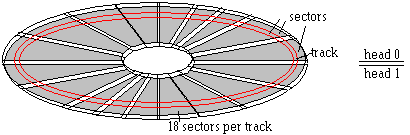
\includegraphics[width=.5\textwidth]{../figs/bootLoader/flpy1.png}
  \caption{Floppy disk structure}
  \label{fig:flpy1.png}
\end{figure}

A floppy disk, also called a floppy, diskette, or just disk, is a type of disk storage
composed of a disk of thin and flexible magnetic storage medium, sealed in a rectangular
plastic enclosure lined with fabric that removes dust particles. Floppy disks are read and
written by a floppy disk drive (FDD)\cite{wiki:floppy}.

For 3.5 inch HD floppy,  There are 80 cylinders from the outermost to
the core on each side, numbering 0, 1, \ldots, 79. The head can assign be 0 or 1,
representing two sides of floppy. When specify head number and cylinder number, forming a
ring, named track in jargon. The track is large so we divide it to 18 small parts, named
sector. A sector can store 512 byte. So the capacity of a floppy is:

\[18 \times 80 \times 2 \times 512 = 1474560\,Byte = 1440\,KiB\]


\chapter{Design}

\section{Top Level Design}


\subsection{32-bit Mode and Import C Codes}

\chapter{Implementation}

\section{Boot Loader}

\subsection{Workflow of Boot Loader}

Fig.~\ref{fig:flowchart-of-boot-loader} shows how the boot loader works.

\begin{figure}[!ht]
  \centering
  % 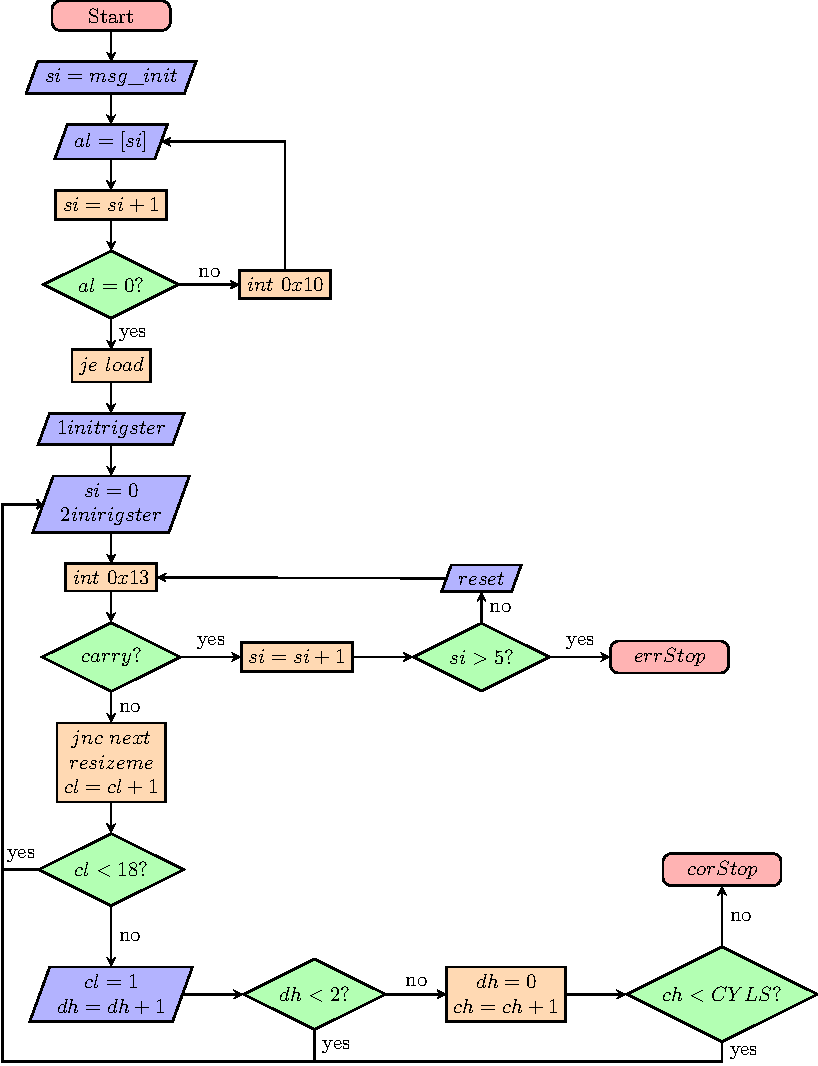
\includegraphics[width=1\textwidth]{../figs/FlowchartTex/1/flowcharte.pdf}
  \fxerror{need a better chart}
  \caption{Flowchart of boot loader}\label{fig:flowchart-of-boot-loader}  
\end{figure}

The boot loader is implemented in Intel assembly. It works as following:

\begin{enumerate}
\item \textbf{Display boot information:} Firstly, the code in boot sector (See
  Appendix~\ref{sec:dis-boo-inf}) outputs some boot information. When \texttt{al=0}, the
  null character of boot information hit. Interrupt \texttt{0x10} is used for showing a
  character.
\item \textbf{Read the second sector:} Then jump to load C0-H0-S2, \texttt{ax} register
  saved the address where beginning puts the sectors from floppy. And preparing parameters
  for interrupt \texttt{0x13} in registers. The \texttt{0x13} interrupt used for read
  sector from floppy to memory. (See Appendix~\ref{sec:rea-sec-sec}).
\item \textbf{Read two sides of a track:} \fxnote{perhaps you should use pseudo-code to
    illustrate these steps.}
  
  If there is a carry indicating some thing went wrong while reading the floppy disk,
  reset the registers and try reading it again. The read process aborts after five
  unsuccessful read.

  Register \texttt{si} is a counter. If no carry (success), jump to next segment, as one
  sector has been read into memory already. The address should increase 512 byte. Then
  sector number (\texttt{cl} register) is added by 1 and compare it to 18, if it's smaller
  than 18, jump to \texttt{readloop}, read the next sector.

  If the value of \texttt{cl} register bigger or equal to than 18, meaning that one track
  18 sector in this side of floppy read already, then reversed the head, add 1 to
  \texttt{dh} register.

  If the value of \texttt{dh} register after adding larger than or equal to 2, it's saying
  the original head is 1, one track of two sides read already. Otherwise the value of
  \texttt{dh} register smaller than 2, read this side indicating by \texttt{dh} register,
  jump to \texttt{readloop} segmentation. Appendix~\ref{sec:rea-two-sid} is the code to
  perform this function.
\item \textbf{The next cylinder:} So the next step is moving a cylinder, add 1 to register
  \texttt{ch}. Otherwise the value of \texttt{dh} register smaller than 2, read this side
  indicating by \texttt{dh} register, jump to \texttt{readloop} segmentation. After
  \texttt{ch} register add 1, if it's smaller than 10, jump to \texttt{readloop},
  otherwise end loading floppy to memory process, for we only load ten cylinders of
  floppy. Appendix~\ref{sec:the-nex-cyl} is the code to perform this function.
\end{enumerate}

\subsection{Running Result}

Fig.~\ref{fig:iplRes} shows the running results of boot loader. From this picture we
see that the boot loader loaded 10 cylinders from floppy successfully. 

\begin{figure}[!ht]
  \centering
  % 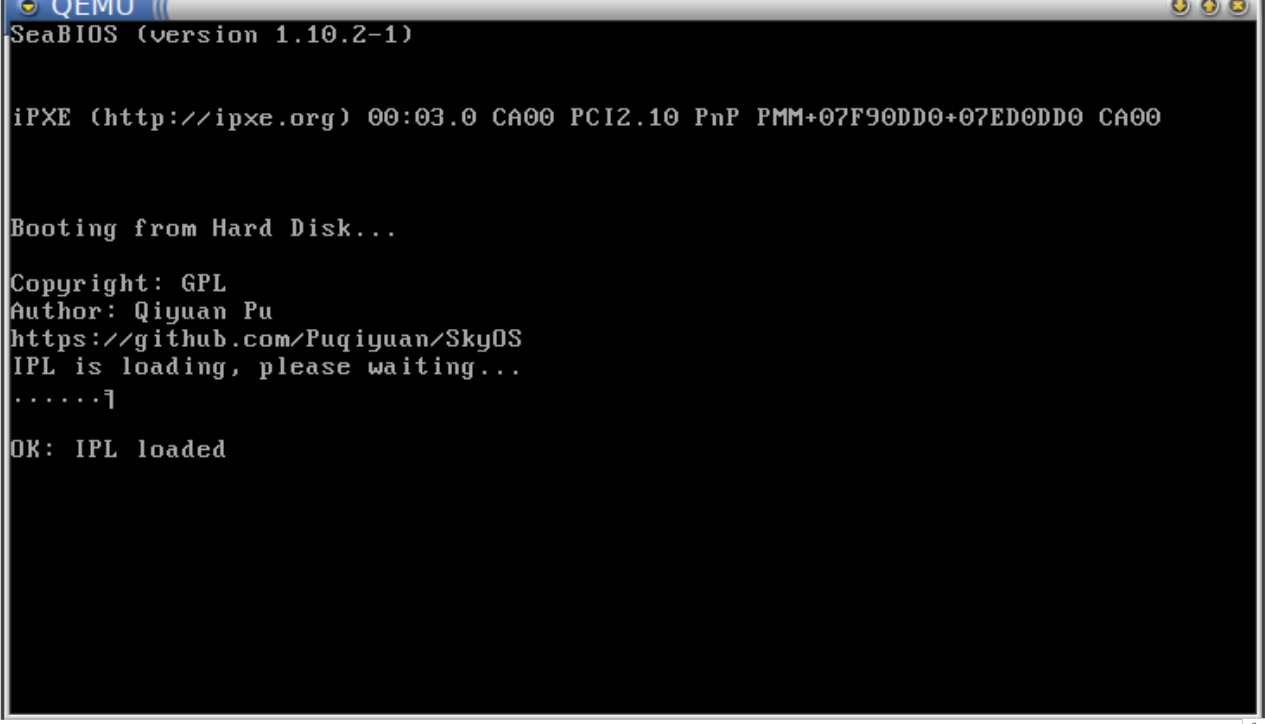
\includegraphics[width=1.1\textwidth]{iplRes.png}
  \fxerror{need a better pic.}
  \caption{Running result of boot loader}\label{fig:iplRes}  
\end{figure}


\section{32-bit Mode and Import C Codes}


\section{Screen Display and Text}

\section{Control Mouse}


\section{Memory Management}

\section{Making Window }

\section{Timer}

\section{Multitasking}

\section{Command Line Window}

\section{API}

\section{OS Protection}

\section{Graphics Processing}

\section{Window Operation}

\section{Application Protection}

\section{File Operation}

\section{Some Applications}

\chapter{Conclusions}%{Prospects And Shortages}

\footnotetext{\url{https://thesistips.wordpress.com/2012/03/25/how-to-write-your-introduction-abstract-and-summary/}}

\paragraph{What goes in your ``Conclusions'' chapter?}

{\fontspec[Scale=.8]{Purisa} The purpose of this chapter is to provide a summary of the
  whole thesis or report.  In this context, it is similar to the Abstract, except that the
  Abstract puts roughly equal weight on all thesis/report chapters, whereas the
  Conclusions chapter focuses primarily on the findings, conclusions and/or
  recommendations of the project.

  There are a couple of rules – one rigid, one common sense, for this chapter:
  \begin{itemize}
  \item All material presented in this chapter must have appeared already in the report;
    no new material can be introduced in this chapter. (rigid rule of technical writing)
  \item Usually, you would not present any new figures or tables in this chapter. (rule of thumb)
  \end{itemize}

  Generally, for most technical reports and Masters theses, the Conclusions chapter would
  be~3 to 5 pages long (double spaced).  It would generally be longer in a large PhD
  thesis. Typically you would have a paragraph or two for each chapter or major
  subsection.  Aim to include the following (typical) content.
  \begin{enumerate}
  \item Re-introduce the project and the need for the work – though more briefly than in
    the intro;
  \item Re-iterate the purpose and specific objectives of your project.
  \item Re-cap the approach taken – similar to the road map in the intro; however, in this
    case, you are re-capping the data, methodology and results as you go.
  \item Summarize the major findings and recommendations of your work.
  \item Make recommendations for future research.
  \end{enumerate}}

%%% 正文部分到此结束。下面是『参考文献』、『指导教师简介』、『鸣谢』、『附录』

%% 不要动下面四行!
\appendix{}
\printbibliography[heading={bibintoc},title={Bibliography}] % 输出参考文献
\advisorinfopage{}                 % 输出指导教师简介
\acknowledgmentspage{}             % 输出鸣谢

%%% 下面是附录部分,可以没有。

\chapter{Main Program Code} %附录一

\section{Boot loader}

\subsection{Display boot information}
\label{sec:dis-boo-inf}

\inputminted[firstline=55, lastline=65,
  linenos=true]{nasm}{../../src/06day/RongC/ipl10.asm}

\subsection{Read the second sector}
\label{sec:rea-sec-sec}
  
\inputminted[firstline=87,lastline=106,linenos=true]{nasm}{../../src/06day/RongC/ipl10.asm}

\subsection{Read two sides of a track}
\label{sec:rea-two-sid}

\inputminted[firstline=108,lastline=132,linenos=true]{nasm}{../../src/06day/RongC/ipl10.asm}

\subsection{The next cylinder}
\label{sec:the-nex-cyl}

\inputminted[firstline=134,lastline=137,linenos=true]{nasm}{../../src/06day/RongC/ipl10.asm}

\end{document} % 结束。不要动下面几行!

%%% Local Variables:
%%% mode: latex
%%% TeX-master: t
%%% End:
